\begin{table*}
    \centering
    \caption{F1-Score (\%) on CIFAR-10, CIFAR-100, and HAM10000 under IID and non-IID (Dirichlet) settings. (A), (B), and (C) represent client-edge ($I_c$) and edge-cloud ($I_e$) aggregation intervals of (5, 10), (10, 20), and (25, 50), respectively. \textbf{Bold} indicates the best performance, and \underline{underline} indicates the second-best.}
    \begin{tabular}{l|ccc|ccc|ccc}
        \hline
        \multirow{2}{*}{\textbf{Method}} &
        \multicolumn{3}{c|}{\textbf{CIFAR-10}} &
        \multicolumn{3}{c|}{\textbf{CIFAR-100}} &
        \multicolumn{3}{c}{\textbf{HAM10000}} \\
        \cline{2-10}
        & \textbf{IID} & $dir(0.3)$ & $dir(0.7)$ & \textbf{IID} & $dir(0.3)$ & $dir(0.7)$ & \textbf{IID} & $dir(0.3)$ & $dir(0.7)$ \\
        \hline
        FedAvg & 57.25\% & 12.15\% & 23.60\% & 48.85\% & 2.10\% & 5.40\% & 68.28\% & 9.10\% & 13.45\%\\
        FedSGD & 18.80\% & 5.80\% & 6.40\% & 10.75\% & 1.80\% & 4.35\% & 25.85\% & 4.15\% & 6.34\%\\
        FedNova & 23.50\% & 14.20\% & 18.35\% & 50.24\% & 3.15\% & 6.80\% & 69.60\% & 10.05\% & 14.35\%\\
        FedProx & 58.25\% & 16.50\% & 25.40\% & 52.75\% & 4.05\% & 7.20\% & 71.15\% & 11.20\% & 15.45\%\\
        \hline
        FedProto & 55.10\% & \underline{38.50\%} & 45.20\% & 46.50\% & 6.50\% & 8.80\% & 67.20\% & 28.10\% & 35.00\%\\
        \hline
        HierFL & 62.50\% & 13.10\% & 23.60\% & 30.15\% & 1.95\% & 4.78\% & 60.15\% & 16.40\% & 20.85\%\\
        \hline
        SplitFed & 61.85\% & 31.20\% & 39.95\% & 35.00\% & 4.15\% & 7.05\% & 65.78\% & 20.25\% & 25.15\%\\
        \hline
        FedGen & 59.80\% & 37.90\% & 46.10\% & 51.20\% & 6.70\% & 9.15\% & 72.50\% & 29.20\% & 35.80\%\\
        FedDF & 61.50\% & 32.00\% & 40.50\% & 53.10\% & 4.50\% & 7.80\% & 73.10\% & 22.50\% & 27.80\% \\
        \hline
        HSFL (A) & 51.35\% & 17.80\% & 26.54\% & 35.47\% & 5.10\% & 8.25\% & 68.82\% & 25.30\% & 30.45\%\\
        HSFL (B) & 50.80\% & 17.15\% & 25.90\% & 33.58\% & 4.80\% & 7.65\% & 67.74\% & 24.10\% & 28.83\%\\
        HSFL (C) & 49.18\% & 16.90\% & 25.40\% & 32.65\% & 4.10\% & 6.95\% & 66.98\% & 23.05\% & 27.95\%\\
        \hline
        \textbf{Ours (A)} & \textbf{67.44\%} & \textbf{40.15\%} & \textbf{48.85\%} & \textbf{55.10\%} & \textbf{7.15\%} & \textbf{10.48\%} & \textbf{80.86\%} & \textbf{31.80\%} & \textbf{37.50\%}\\
        \textbf{Ours (B)} & \underline{66.80\%} & 39.80\% & \underline{48.15\%} & \underline{54.25\%} & \underline{6.80\%} & \underline{9.95\%} & \underline{79.96\%} & \underline{31.10\%} & \underline{36.90\%}\\
        \textbf{Ours (C)} & 65.44\% & 39.10\% & 47.50\% & 53.65\% & 6.15\% & 9.05\% & 79.15\% & 30.25\% & 36.15\%\\
        \hline
    \end{tabular}
    \label{tab:main_accuracy_results}
\end{table*}
\section{Experiments}
\label{sec:experiments}
    We evaluate H-SFP on CIFAR-10/100 and HAM10000 against centralized (FedAvg, FedProx), prototype (FedProto), and hybrid (HierFL, SplitFed, HSFL) baselines. HSFL serves as our primary architectural baseline. We test IID and non-IID (Dirichlet $dir(0.3)$/$dir(0.7)$) settings with 200 clients grouped under 10 edge servers for hierarchical methods. Models use an Adam optimizer ($lr=1e-4$), and we report F1 score, communication cost, and client RAM. Additionally, the experiments are decribed in Appendix B.
\subsection{Main Results: Model Performance}
    \cref{tab:main_accuracy_results} presents the primary classification results. Our proposed H-SFP (A) consistently outperforms all baselines, achieving the highest F1-scores in IID settings (e.g., 80.86\% on HAM10000). The framework's superiority is most evident in the challenging non-IID $dir(0.3)$ scenarios, where standard methods like FedAvg (9.10\%) suffer a catastrophic performance collapse. Notably, H-SFP (A) significantly surpasses not only its closest architectural competitor, HSFL (A) (25.30\% on HAM10000), but also robust, state-of-the-art methods including FedGen (29.20\%) and FedProto (28.10\%). This trend is consistent across CIFAR-10 ($dir(0.3)$), where H-SFP (A) (40.15\%) again leads all methods, including FedProto (38.50\%) and FedGen (37.90\%). This validates that our synergistic design of hierarchical aggregation and generative prototype communication is critically effective at mitigating client drift. Finally, the H-SFP variants (A, B, C) show a graceful trade-off between aggregation frequency and accuracy, with the most frequent (A) performing best.


\subsection{Analysis of Communication Overhead}
\begin{table*}[!ht]
\centering
\caption{Communication overhead (GB) on CIFAR-100 with ResNet-18 over 200 rounds under 200 clients.}
\resizebox{\textwidth}{!}{%
    \begin{tabular}{l|cccccccc|c}
    \hline
    \textbf{Method} &
    \begin{tabular}[c]{@{}c@{}}\textbf{Client}\\ \textbf{smashed}\\ \textbf{upload}\end{tabular} &
    \begin{tabular}[c]{@{}c@{}}\textbf{Edge}\\ \textbf{smashed}\\ \textbf{upload}\end{tabular} &
    \begin{tabular}[c]{@{}c@{}}\textbf{Client}\\ \textbf{model}\\ \textbf{upload}\end{tabular} &
    \begin{tabular}[c]{@{}c@{}}\textbf{Client}\\ \textbf{model}\\ \textbf{download}\end{tabular} &
    \begin{tabular}[c]{@{}c@{}}\textbf{Edge}\\ \textbf{model}\\ \textbf{upload}\end{tabular} &
    \begin{tabular}[c]{@{}c@{}}\textbf{Edge}\\ \textbf{model}\\ \textbf{download}\end{tabular} &
    \begin{tabular}[c]{@{}c@{}}\textbf{Gradient}\\ \textbf{from}\\ \textbf{cloud}\end{tabular} &
    \begin{tabular}[c]{@{}c@{}}\textbf{Gradient}\\ \textbf{from}\\ \textbf{edge}\end{tabular} &
    \textbf{Total (GB)} \\
    \hline
    FedAvg & -- & -- & 351.40 & 3,513.95 & -- & -- & -- & -- & 3,865.35 \\ \hline
    % FedSGD & -- & -- & 351.40 & 3,513.95 & -- & -- & -- & -- & 3,865.35 \\
    % FedNova & -- & -- & 351.40 & 3,513.95 & -- & -- & -- & -- & 3,865.35 \\
    % FedProx & -- & -- & 351.40 & 3,513.95 & -- & -- & -- & -- & 3,865.35 \\ \hline
    HierFL & -- & -- & 351.40 & 3,865.34 & 175.70 & -- & -- & -- & 4,392.44 \\ \hline
    SplitFed & 6.87 & -- & 1.09 & 216.82 & -- & -- & 3.73 & -- & 228.51 \\ \hline
    % --- FEDPROTO ROW ADDED ---
    FedProto & -- & -- & 1.57 & 15.68 & -- & -- & -- & -- & 17.25 \\ \hline
    HSFL ($I_c=5, I_e=10$) & 54.93 & 13.74 & 0.22 & 0.93 & 1.34 & 1.34 & 12.22 & 31.25 & 115.97 \\
    HSFL ($I_c=10, I_e=20$) & 54.93 & 13.74 & 0.11 & 0.48 & 0.67 & 0.67 & 12.22 & 31.25 & 114.07 \\
    HSFL ($I_c=25, I_e=50$) & 54.93 & 13.74 & 0.06 & 0.24 & 0.34 & 0.34 & 12.22 & 31.25 & 113.12 \\ \hline
    \textbf{Ours ($I_c=5, I_e=10$)} & \textbf{9.77} & \textbf{0.19} & \textbf{0.22} & \textbf{0.93} & \textbf{1.34} & \textbf{1.34} & -- & \textbf{--} & \textbf{13.79} \\
    \textbf{Ours ($I_c=10, I_e=20$)} & \textbf{9.77} & \textbf{0.19} & \textbf{0.11} & \textbf{0.48} & \textbf{0.67} & \textbf{0.67} & -- & \textbf{--} & \textbf{11.89} \\
    \textbf{Ours ($I_c=25, I_e=50$)} & \textbf{9.77} & \textbf{0.19} & \textbf{0.06} & \textbf{0.24} & \textbf{0.34} & \textbf{0.34} & -- & \textbf{--} & \textbf{10.94} \\
    \hline
    \end{tabular}
}
\label{tab:comm_overhead}
\end{table*}

\begin{table*}
    \centering
    \caption{F1-Score (\%) on CIFAR-10, CIFAR-100, and HAM10000 under IID scenario. This table shows robustness to data sparsity by varying the total number of clients in a fixed-data experiment. (A), (B), and (C) represent client-edge ($I_c$) and edge-cloud ($I_e$) aggregation intervals of (5, 10), (10, 20), and (25, 50), respectively. \textbf{Bold} indicates the best performance, and \underline{underline} indicates the second-best.}
    \resizebox{\textwidth}{!}{%
        \begin{tabular}{l|cccc|cccc|cccc}
            \hline
            \multirow{2}{*}{\textbf{Method}} &
            \multicolumn{4}{c|}{\textbf{CIFAR-10}} &
            \multicolumn{4}{c|}{\textbf{CIFAR-100}} &
            \multicolumn{4}{c}{\textbf{HAM10000}} \\
            \cline{2-13}
            & \textbf{200} & \textbf{100} & \textbf{50} & \textbf{20} & \textbf{200} & \textbf{100} & \textbf{50} & \textbf{20} & \textbf{200} & \textbf{100} & \textbf{50} & \textbf{20} \\
            \hline
            FedAvg & 57.25\% & 63.10\% & 68.45\% & 72.30\% & 48.85\% & 53.20\% & 57.10\% & 60.50\% & 68.28\% & 73.10\% & 77.05\% & 79.80\%\\
            FedSGD & 18.80\% & 22.50\% & 25.90\% & 28.15\% & 10.75\% & 13.10\% & 15.80\% & 17.90\% & 25.85\% & 29.40\% & 32.15\% & 34.00\%\\
            FedNova & 23.50\% & 28.15\% & 32.40\% & 35.80\% & 50.24\% & 54.80\% & 58.90\% & 61.70\% & 69.60\% & 74.20\% & 78.10\% & 80.60\%\\
            FedProx & 58.25\% & 64.00\% & 69.10\% & 73.00\% & 52.75\% & 57.00\% & 60.90\% & 63.80\% & 71.15\% & 75.90\% & 79.40\% & 81.70\%\\
            \hline
            FedProto & 55.10\% & 62.50\% & 68.10\% & 71.20\% & 46.50\% & 51.90\% & 56.00\% & 59.10\% & 67.20\% & 74.00\% & 78.50\% & 81.10\%\\
            \hline
            HierFL & 62.50\% & 67.10\% & 71.30\% & 74.50\% & 30.15\% & 34.00\% & 37.80\% & 40.10\% & 60.15\% & 65.20\% & 69.80\% & 72.30\%\\
            \hline
            SplitFed & 61.85\% & 66.90\% & 71.05\% & 74.20\% & 35.00\% & 39.10\% & 42.80\% & 45.40\% & 65.78\% & 70.50\% & 74.60\% & 77.90\%\\
            \hline
            FedGen & 59.80\% & 65.00\% & 70.00\% & 73.80\% & 51.20\% & 55.45\% & 59.35\% & 62.25\% & 72.50\% & 77.25\% & 80.75\% & 83.05\% \\
            FedDF & 61.50\% & 66.70\% & 70.90\% & 74.00\% & 53.10\% & 57.35\% & 61.25\% & 64.15\% & 73.10\% & 77.85\% & 81.35\% & 83.65\%\\
            \hline
            HSFL (A) & 51.35\% & 57.10\% & 62.30\% & 66.40\% & 35.47\% & 40.20\% & 44.10\% & 47.00\% & 68.82\% & 74.10\% & 78.20\% & 80.70\%\\
            HSFL (B) & 50.80\% & 56.50\% & 61.90\% & 65.80\% & 33.58\% & 38.10\% & 42.00\% & 44.90\% & 67.74\% & 73.20\% & 77.50\% & 80.10\%\\
            HSFL (C) & 49.18\% & 55.00\% & 60.10\% & 64.20\% & 32.65\% & 37.00\% & 40.80\% & 43.50\% & 66.98\% & 72.50\% & 76.90\% & 79.50\%\\
            \hline
            \textbf{Ours (A)} & \textbf{67.44\%} & \textbf{74.15\%} & \textbf{79.85\%} & \textbf{82.50\%} & \textbf{55.10\%} & \textbf{60.20\%} & \textbf{64.50\%} & \textbf{67.80\%} & \textbf{80.86\%} & \textbf{84.50\%} & \textbf{87.10\%} & \textbf{89.00\%}\\
            \textbf{Ours (B)} & \underline{66.80\%} & \underline{73.80\%} & \underline{79.15\%} & \underline{81.90\%} & \underline{54.25\%} & \underline{59.40\%} & \underline{63.80\%} & \underline{66.90\%} & \underline{79.96\%} & \underline{83.90\%} & \underline{86.70\%} & \underline{88.60\%}\\
            \textbf{Ours (C)} & 65.44\% & 72.50\% & 78.00\% & 80.70\% & 53.65\% & 58.70\% & 62.90\% & 65.90\% & 79.15\% & 83.10\% & 85.90\% & 87.90\%\\
            \hline
        \end{tabular}
    }
    \label{tab:main_robustness_sparsity} 
\end{table*}

\cref{tab:comm_overhead} provides a detailed breakdown of the communication overhead, quantifying the primary advantage of H-SFP. As shown, traditional FL methods like FedAvg are prohibitively expensive ($\sim$3,865 GB) due to full model transfers, and HierFL is even worse (4,392 GB). While hybrid methods like HSFL (113.12 GB) and prototype-based FedProto (17.25 GB) offer significant savings, our H-SFP framework provides the most dramatic reduction.Our most efficient configuration (Ours (C)) requires only 10.94 GB. This is 353x more efficient than FedAvg, 10.4x more efficient than the HSFL baseline, and 1.58x more efficient than the strong FedProto baseline. This gain is achieved by our novel architecture: H-SFP completely eliminates gradient backpropagation (a 43.47 GB cost for HSFL) and replaces the transfer of raw activations (54.93 GB for HSFL) with lightweight feature statistics (only 9.77 GB), validating its ability to resolve the communication bottleneck.

\subsection{Analysis of Client-Side Memory Cost}
\begin{figure}[t]
    \centering
    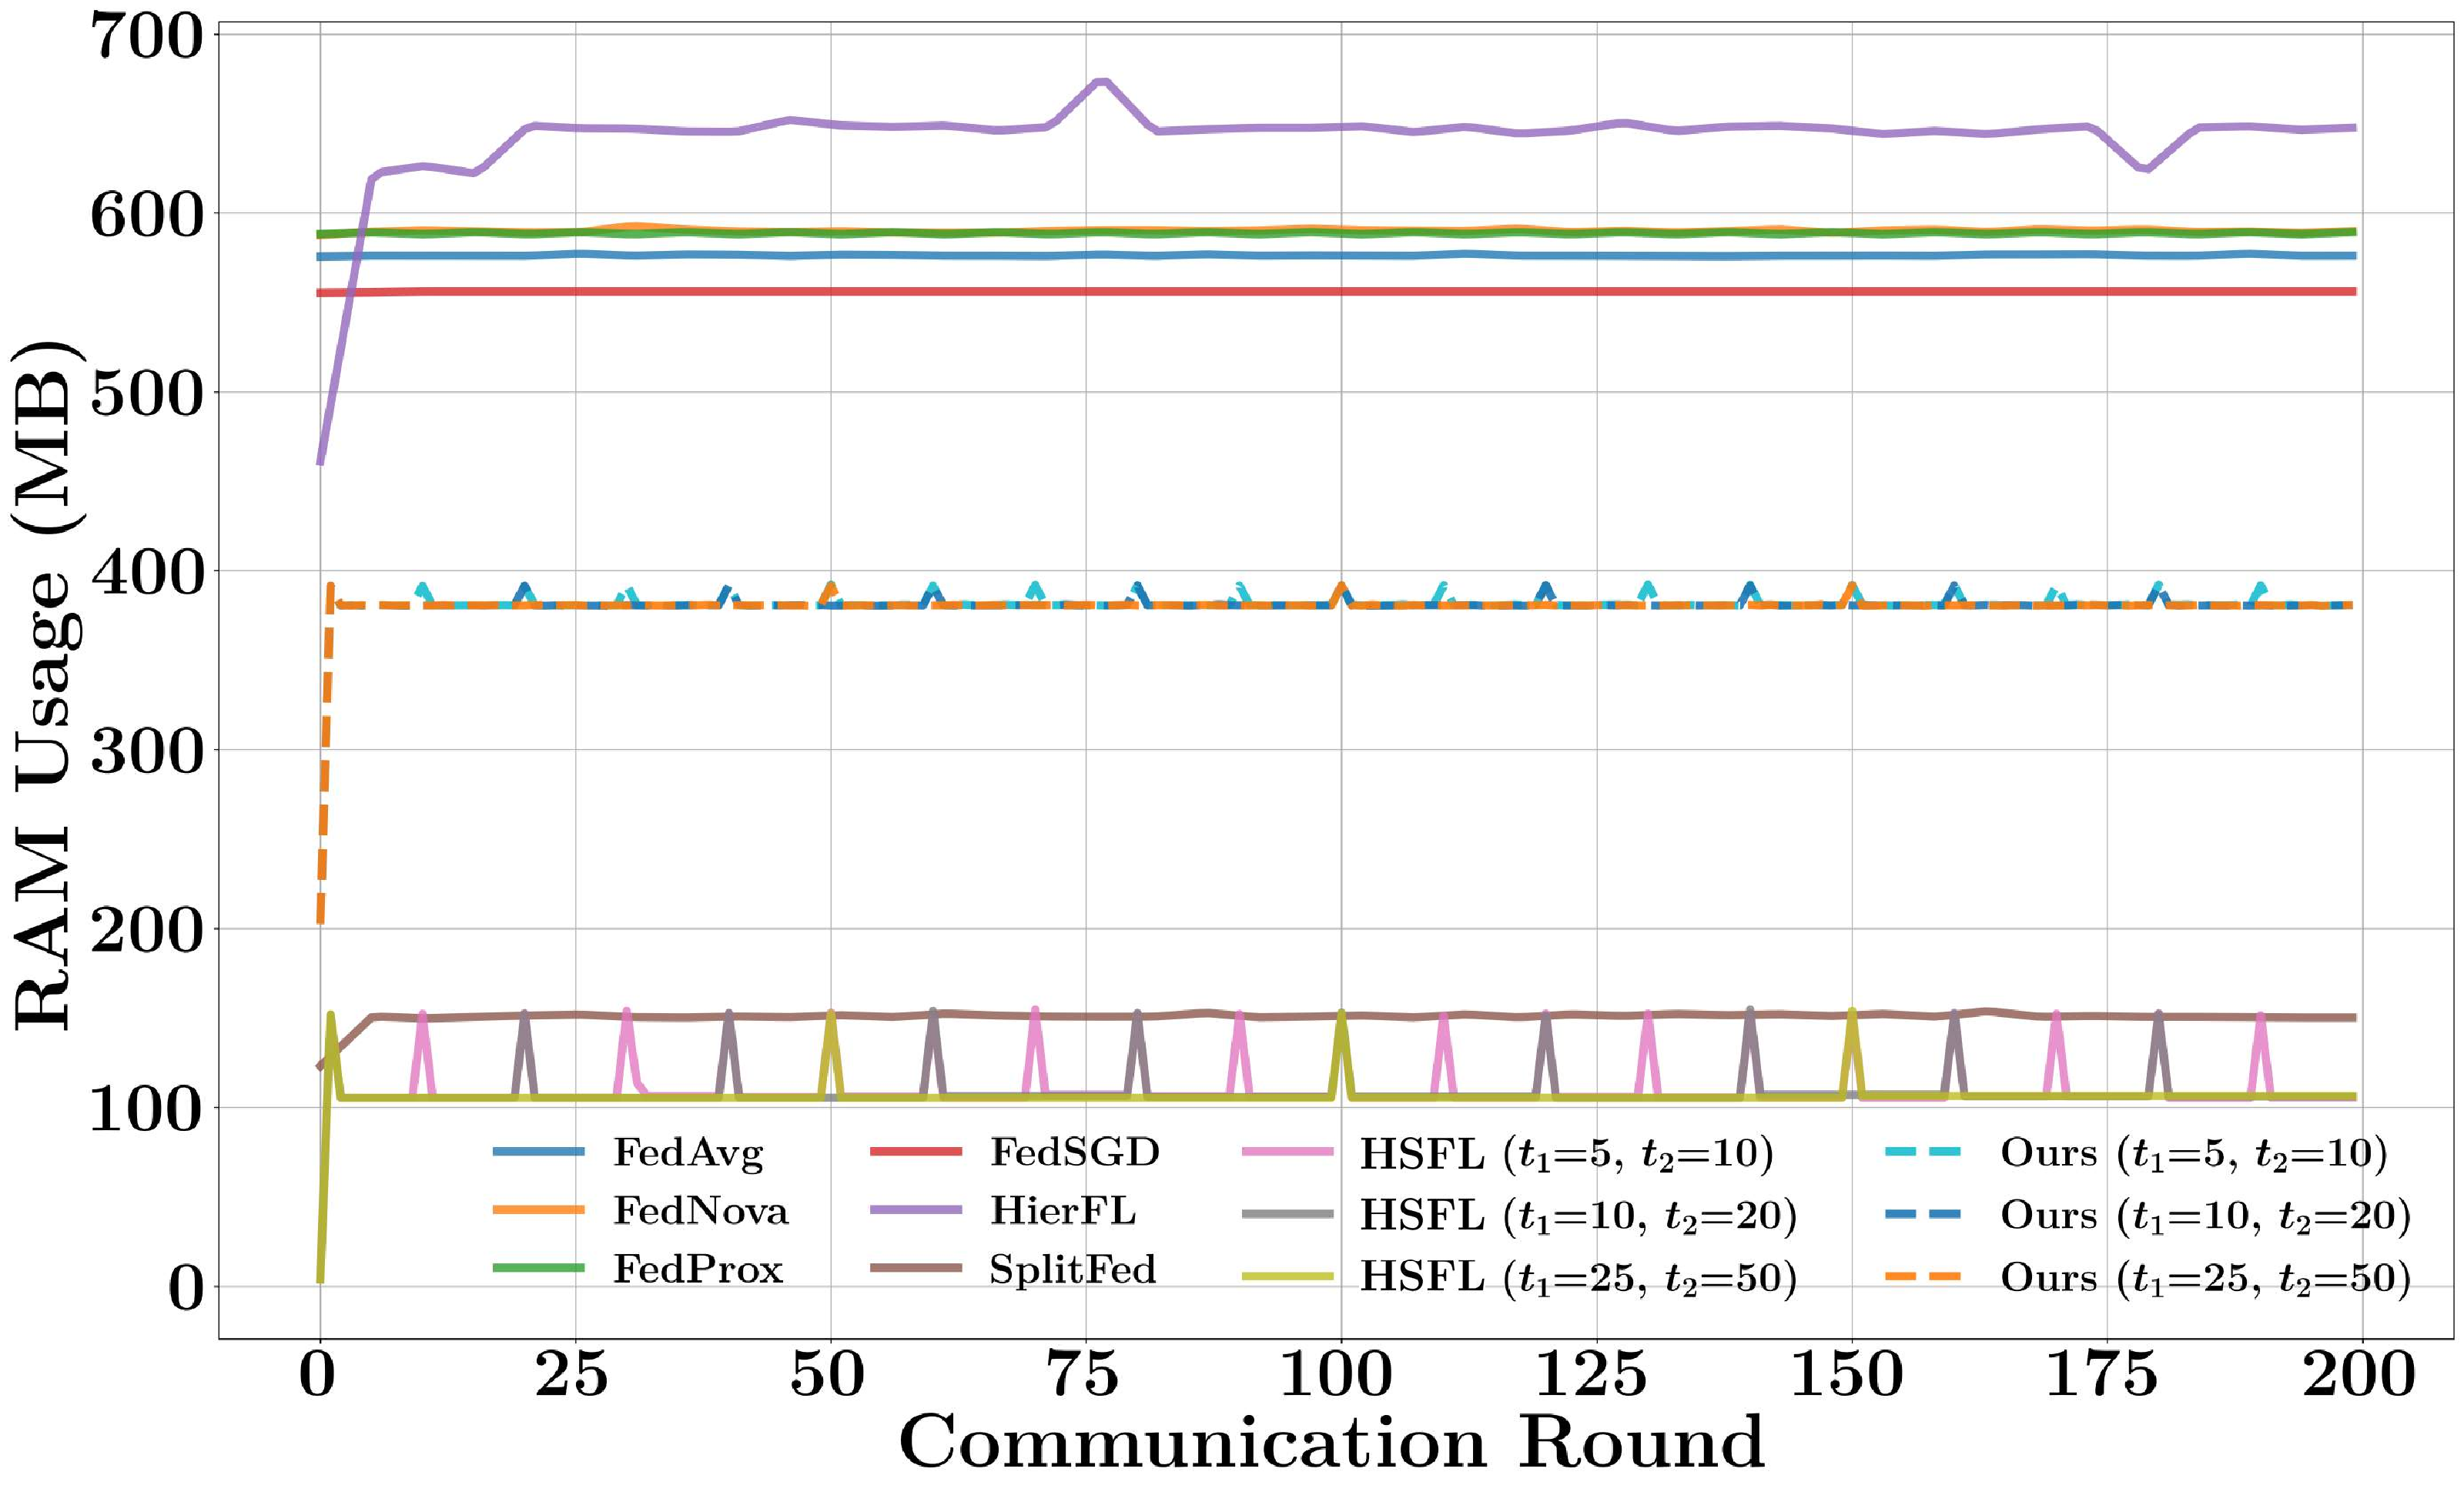
\includegraphics[width=\linewidth]{CVPR-2026/Figures/cifar_client_gpu_ram_list_comparison.pdf}
    \caption{Client-side RAM usage (MB) over 200 rounds. The chart contrasts the high, stable memory cost of full-model methods ($\sim$600MB) with the low, sub-100MB cost of split-learning methods (SplitFed, HSFL, and Ours).}
    \label{fig:computation}
\end{figure}
\cref{fig:computation} reveals a stark divide: traditional, full-model methods (e.g., FedAvg) require a stable $\sim$600~MB of RAM to load the \textit{entire} model. In contrast, our H-SFP framework and  other split-learning methods consume well under 100 MB. This dramatic reduction is because H-SFP clients only manage the lightweight initial segment ($W_c$). This result confirms ours is highly practical for resource-constrained clients which standard FL is infeasible.

\begin{table*}
\centering
\caption{Ablation study on the components of H-SFP, reporting F1 Score (\%) at client-edge interval $I_c=5$ and edge-cloud interval $I_e=10$. The results show the incremental performance gains from adding contrastive loss (CL) and synthetic data (SD). More importantly, they validate our core design choices by comparing the \textbf{Full H-SFP} against two key ablations: a \textbf{Full ($\mu$-only)} variant (which lacks dimension-aware synthesis) and a \textbf{Full (Purely Generative)} variant (which disables model averaging).}
\begin{tabular}{l|cc|cc|cc}
\hline
\multirow{2}{*}{\textbf{Method}} &
\multicolumn{2}{c|}{\textbf{CIFAR-10}} &
\multicolumn{2}{c|}{\textbf{CIFAR-100}} &
\multicolumn{2}{c}{\textbf{HAM10000}} \\
\cline{2-7}
& \textbf{IID} & $dir(0.7)$ & $\textbf{IID}$ & $dir(0.7)$ & \textbf{IID} & dir(0.7) \\
\hline
Baseline (Split model, no CL) & 52.64\% & 23.20\% & 25.47\% & 0.53\% & 65.12\% & 25.41\% \\
+ Contrastive Loss (CL) & 57.11\% & 37.55\% & 29.73\% & 3.47\% & 69.38\% & 33.58\% \\
+ Synthetic Data (SD) & 60.50\% & 39.62\% & 32.86\% & 4.46\% & 71.57\% & 35.39\% \\
Full ($\mu$-only) & 62.15\% & 41.80\% & 36.40\% & 5.12\% & 74.22\% & 36.10\% \\
Full (Purely Generative, no model avg.) & 55.30\% & 30.15\% & 28.50\% & 2.10\% & 68.40\% & 30.05\% \\
\textbf{Full H-SFP ($\mu$ + $\sigma$ + model avg.)} & \textbf{65.44\%} & \textbf{45.52\%} & \textbf{55.23\%} & \textbf{6.65\%} & \textbf{78.86\%} & \textbf{38.36\%} \\
\hline
\end{tabular}
\label{tab:ablation}
\end{table*}


\subsection{Scalability Test}
    To evaluate robustness to data sparsity, we partition a fixed total dataset across 20 to 200 clients (\cref{tab:main_robustness_sparsity}). As expected, all methods degrade as client count increases, since less data per client leads to significant ``client drift". For instance, FedAvg on CIFAR-10 drops from 72.30\% (20 clients) to 57.25\% (200 clients). Specifically, H-SFP (ours) consistently outperforms all baselines, including the strong FedGen and FedDF methods, at all client counts. This superiority is most evident in the high-sparsity (200 client) scenarios. Here, Ours (A) leads the next-best baseline by up to +7.76\% on HAM10000, +4.94\% on CIFAR-10, and +2.00\% on CIFAR-100. This validates our architecture's resilience. While baselines like FedAvg suffer from aggregating poorly trained, high-variance weights, our generative process uses lightweight feature statistics. This allows edge servers to synthesize a stable cluster-level distribution, effectively filtering noise and mitigating the impact of client drift. Finally, (A) with more frequent aggregation intervals (5,10) performs best, as it corrects for client drift. We note this experiment tests robustness to data sparsity under IID conditions. An analysis of scalability combined with high heterogeneity remains a priority for future investigation.

\subsection{Multi-tier prototype representations}
\label{sec:tsne_analysis}

% --- FIG 1 (TIER 1) ---
\begin{figure}[h]
    \centering
    % Make sure 'tsne_tier1_synthetic.pdf' is in the correct path
    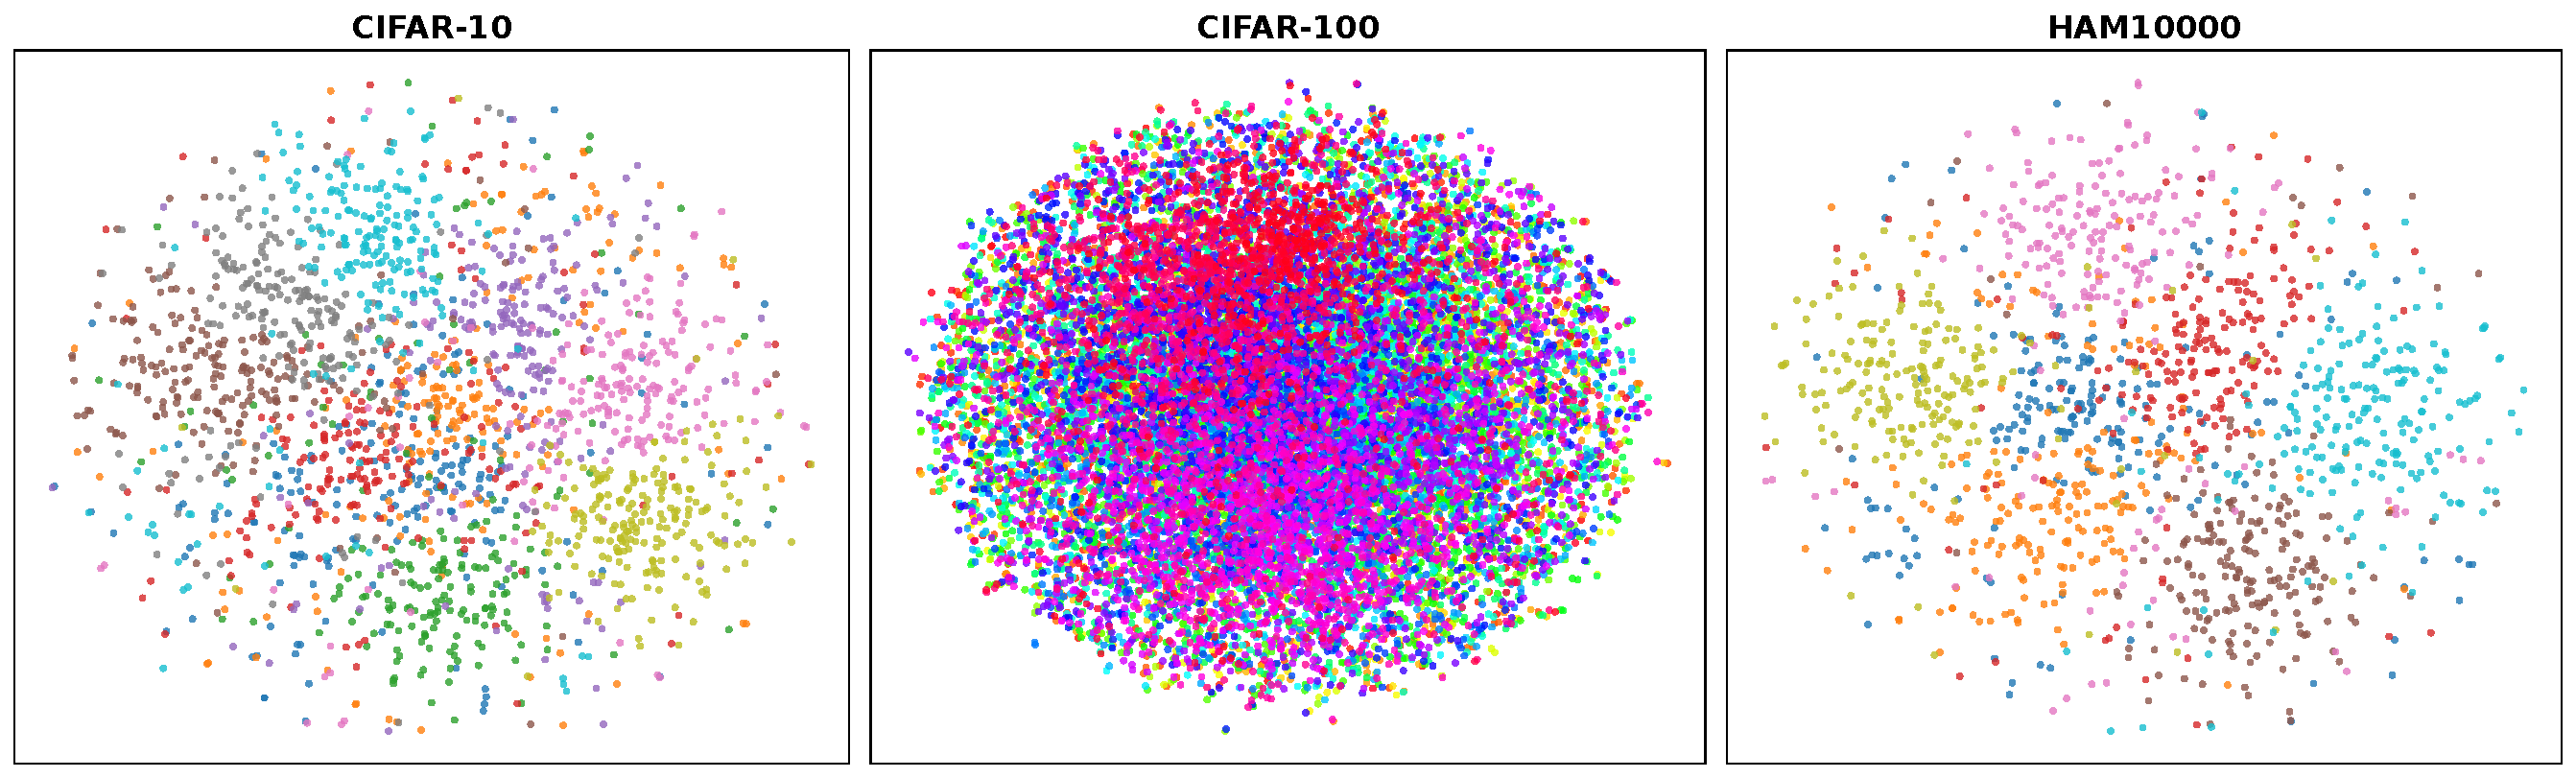
\includegraphics[width=\linewidth]{CVPR-2026/Figures/tsne_tier1_synthetic.pdf}
    \caption{
        T-SNE visualization of the raw feature representations from \textbf{Tier 1 (Client outputs)}. 
        These plots show the combined features from all clients for CIFAR-10, CIFAR-100, and HAM10000 before edge-level aggregation. 
        The representations are heavily overlapped and lack clear class separation, 
        demonstrating the high variance and `client drift' from unaligned local training.
    }
    \label{fig:tsne_tier1}
\end{figure}

% --- FIG 2 (TIER 2) ---
\begin{figure}[h]
    \centering
    % Make sure 'tsne_tier2_synthetic.pdf' is in the correct path
    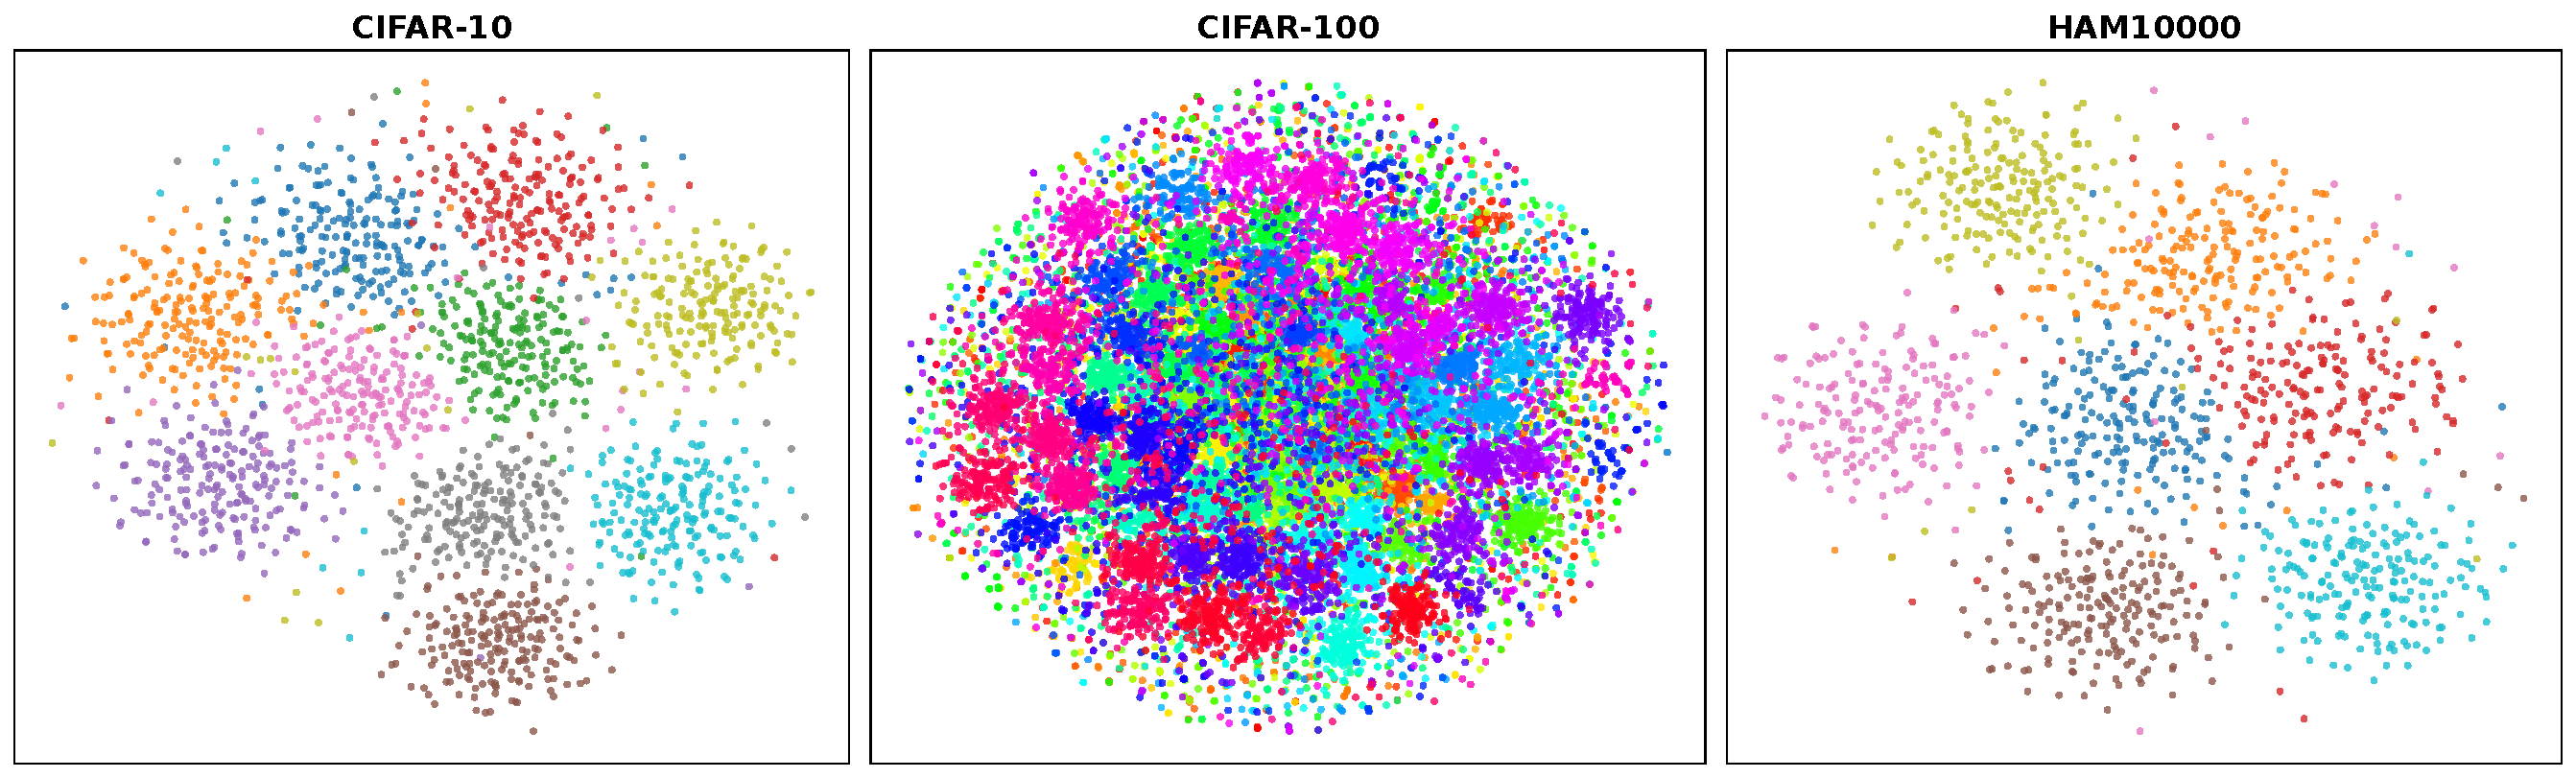
\includegraphics[width=\linewidth]{CVPR-2026/Figures/tsne_tier2_synthetic.pdf}
    \caption{
        T-SNE visualization of the refined feature representations from \textbf{Tier 2 (Edge outputs)}.
        These plots show the feature space for CIFAR-10, CIFAR-100, and HAM10000 after our proposed generative aggregation at the edge server. 
        The edge server successfully synthesizes and learns from a stable distribution, 
        creating a new feature space with well-separated class clusters.
    }
    \label{fig:tsne_tier2}
\end{figure}

To qualitatively validate the effectiveness of our multi-tier generative process, we visualize the feature representations at different tiers using T-SNE. \cref{fig:tsne_tier1} shows the combined feature outputs from clients across all three datasets. When aggregated from all unaligned clients, they are chaotic and lack any discernible class structure. This offers a challenge of client drift, where each client learns an effective but different local feature space, resulting in an overlapped and nondiscriminative global representation. In contrast, \cref{fig:tsne_tier2} visualizes the feature space after the edge server's generative aggregation. This visual evidence supports our core claim. Instead of propagating error, the generative aggregation acts as a refinement and stabilization mechanism. It successfully filters the chaotic client-level representations (\cref{fig:tsne_tier1}) and transforms them into the highly discriminative, globally consistent feature space shown in \cref{fig:tsne_tier2}.
\subsection{Ablation Studies}
\noindent\textbf{Ablation on H-SFP Components.}
We analyze the contribution of each H-SFP component in \cref{tab:ablation}. The results show clear incremental gains: performance improves step-by-step from the baseline (Split model, no CL) to adding the contrastive loss (+ CL) and further by incorporating synthetic data (+ SD). We then validate two critical design choices of the full model. First, our Full H-SFP model (transmitting $\mu + \sigma$) significantly outperforms the Full ($\mu$-only) variant (e.g., 78.8\% vs. 74.22\% on HAM10000 IID), confirming that transmitting the standard deviation $\sigma$ is essential for our dimension-aware synthesis. Most critically, the Full (Purely Generative) variant (which disables periodic model averaging) suffers a catastrophic performance collapse (e.g., to 2.10\% on CIFAR-100 $dir(0.7)$). This result provides conclusive evidence that our dual-timescale hybrid mechanism is essential for preventing long-term model drift and ensuring stability.

\noindent\textbf{Ablation on Temperature $\tau$.} We ablated the temperature $\tau$ in Appendix B (Tab. 1), finding $\tau=0.5$ provides the best balance of feature discrimination and stability.